\documentclass[10pt,twocolumn]{article}

\usepackage[T1]{fontenc}
\usepackage[utf8]{inputenc}
\usepackage{lmodern}
\usepackage{microtype}
\usepackage{graphicx}
\usepackage{booktabs}
\usepackage{tabularx}
\usepackage{array}
\usepackage{amsmath}
\usepackage{amssymb}
\usepackage{siunitx}
\usepackage{subcaption}
\usepackage[colorlinks=true,linkcolor=blue,citecolor=blue,urlcolor=blue]{hyperref}
\captionsetup{hypcap=false}

\sisetup{
  round-mode=places,
  round-precision=3,
  detect-all
}

\title{\textbf{Adaptive Quality Mask Harvesting for Pixel-Wise Quality-Weighted Deep-Sky Reconstruction}\\
\large Method specification, implementation constraints, and an M31-A run}
\author{Jeamy Lee$^{1}$ \\ \small $^{1}$Independent Researcher / tile\_compile project}
\date{June 11, 2026}

\begin{document}
\twocolumn[
\maketitle

\begin{center}
\begin{minipage}{0.88\textwidth}
\small
\textbf{Abstract}\par
\vspace{0.35em}
Adaptive Quality Mask Harvesting (AQMH) is a pixel-wise quality-weighted reconstruction method
for short-exposure deep-sky imaging. It replaces coarse tile-local quality scores with dense
per-frame quality maps and reconstructs each supported output pixel by a deterministic weighted
mean whose AQMH weight is evaluated at the same pixel. The method is independent of Classic Tile
Compile: registration, normalization, common overlap, reporting, and run management may be shared,
but AQMH does not use classic local tile metrics, state clustering, or synthetic frames as
reconstruction inputs or fallbacks.
This paper consolidates the AQMH v0.1.0 method, describes the implementation contract used by
tile\_compile, and evaluates a concrete M31-A run from 2026-06-11. The run processed 645 frames
on a $3924\times2310$ canvas, wrote 645 dense quality maps at half resolution, and reconstructed
the image with \num{5.699e9} finite map samples, zero missing map samples, zero unsupported
pixels, and no fallback to classic tile weights. The measured median FWHM improved from
\num{12.351} px to \num{5.271} px, corresponding to \num{57.327}\% improvement; background RMS
changed from \num{4.185} to \num{0.714}, a \num{-82.932}\% change.
\end{minipage}
\end{center}

\vspace{0.35cm}
\noindent \textbf{Keywords:} astronomical image reconstruction, deep-sky imaging,
quality maps, pixel-wise weighted mean, short exposure stacking, deterministic reconstruction
\vspace{0.6cm}
]

\section{Introduction}

Short-exposure deep-sky imaging collects many noisy frames instead of a small number of long
exposures. The data contain useful signal even when individual frames suffer from local defects:
cloud edges, satellite traces, registration remnants, small hot-pixel clusters, or spatially
varying seeing. A single global frame score cannot model this spatial variation. Coarse tile
scores improve locality, but they still assign one scalar quality value to an extended region.
This produces two limitations: small artifacts can depress a large block, and constant weights
inside adjacent blocks can introduce discontinuities.

AQMH is documented here as an independent reconstruction path within the tile\_compile project.
The reference method for Classic Tile Compile is
\href{https://doi.org/10.5281/zenodo.19437794}{\emph{Tile-Based Quality Reconstruction for DSO},
Version 3.3.9}.

AQMH addresses this by computing a dense quality field
$Q_{f,c}^{map}(x,y)$ for each frame $f$ and channel or stream $c$. The reconstruction then uses
the frame sample itself and the AQMH weight field at the same pixel:
\begin{equation}
  R_c(p) =
  \frac{\sum_f W_{f,c}^{aqmh}(p) I_{f,c}(p)}
       {\sum_f W_{f,c}^{aqmh}(p)} ,
  \quad W_{f,c}^{aqmh}(p) \ge 0 .
\end{equation}
This keeps the reconstruction core a deterministic weighted mean after the weights have been
computed. AQMH therefore does not hallucinate pixel values, does not synthesize replacement
frames, and does not rely on tile clustering.

\section{Method overview}

\subsection{Inputs and independence}

AQMH reuses only shared preprocessing outputs:
\begin{itemize}
  \item calibrated, registered, prewarped, and normalized frames;
  \item a canvas-valid/common-overlap mask;
  \item global frame diagnostics used for a frame-level weight;
  \item run management, artifacts, reports, and UI status.
\end{itemize}
It is otherwise independent from Classic Tile Compile. In particular, the run studied here
reports \texttt{classic\_tile\_weights\_used=false} and
\texttt{fallback\_to\_classic=false}. The classic phases \texttt{STATE\_CLUSTERING} and
\texttt{SYNTHETIC\_FRAMES} are not part of AQMH reconstruction.

\subsection{Binding invariants}

The AQMH implementation follows five practical invariants:
\begin{enumerate}
  \item No frame is discarded solely because of its AQMH quality map.
  \item Canvas-invalid pixels are excluded from all map and reconstruction statistics.
  \item Once weights are known, reconstruction is a linear weighted mean of finite samples.
  \item Quality maps and diagnostics are deterministic for identical input data and parameters.
  \item AQMH outputs weights, masks, and diagnostics only; it does not predict missing signal.
\end{enumerate}
The M31-A run uses \texttt{cherry\_pick\_enabled=false}; therefore no optional pixel-level
frame subset mode is active.

\subsection{Quality-map model}

For a normalized registered input frame $I_{f,c}(x,y)$, AQMH computes a multi-scale quality
field. At each scale $s$, three local signals are evaluated over valid canvas support:
\begin{itemize}
  \item a sharpness signal based on local Laplacian-response variance;
  \item a local SNR signal based on background-centered positive signal over robust scale;
  \item an artifact anomaly gate based on high-pass outlier fraction.
\end{itemize}
The sharpness and SNR signals are normalized within a frame by robust z-scores and combined by a
sigmoid:
\begin{equation}
\begin{split}
  \Psi_s(x,y) &=
  \sigma\!\left(
    w_{sharp} z(\Phi_{sharp,s})
    + w_{snr} z(\Phi_{snr,s})
  \right) \\
  &\quad \times \Phi_{artifact,s}(x,y).
\end{split}
\end{equation}
Scale maps are upsampled with valid-support interpolation and fused by geometric mean:
\begin{equation}
  Q_{f,c}^{map}(x,y) =
  \left(\prod_{s \in S_{actual}} \Psi_s^{up}(x,y)\right)^{1/|S_{actual}|}.
\end{equation}
The geometric mean is intentionally conservative: one poor scale suppresses the fused quality
at that location. Canvas-invalid pixels are set to zero only as an output convention after they
have already been excluded from all statistics.

\subsection{Reconstruction}

The effective AQMH weight multiplies the frame-level quality term and the spatial quality map:
\begin{equation}
  \begin{split}
  W_{f,c}^{aqmh}(x,y) &=
  G_{f,c}Q_{f,c}^{map}(x,y).
  \end{split}
\end{equation}
For each output pixel, the implementation accumulates finite, canvas-valid samples only. Missing
quality maps are not replaced by unweighted mean contributions. A zero quality map is an
explicit veto for that frame/pixel contribution.

\section{Implementation run}

\subsection{Data and configuration}

The evaluation data are taken from the tile\_compile run on the analysis workstation:
\begin{center}
\small
\path{tile_compile_cpp/runs/M31-A_20260611_193628}
\end{center}
The paper bundle itself is archived under
\href{https://github.com/jeamy/tile_compile/tree/master/docs/AQMH/zenodo-0.1.0}
{\path{docs/AQMH/zenodo-0.1.0}} in the project repository. Run artifacts used for
the measurements are local analysis outputs located in:
\begin{center}
\small
\path{tile_compile_cpp/runs/M31-A_20260611_193628/artifacts}
\end{center}
The final preview shown in Figure~\ref{fig:preview} is derived from
\path{outputs/stacked_rgb_hms.fits}.

\begin{table}[t]
\centering
\caption{M31-A run geometry and frame counts.}
\begin{tabular}{lr}
\toprule
Quantity & Value \\
\midrule
Input frames loaded & 645 \\
Usable frames & 645 \\
Canvas size & $3924\times2310$ px \\
Common-overlap fraction & \num{0.9748} \\
Reconstruction fraction & \num{0.9823} \\
Adaptive tiles in shared grid & 209 \\
Tile size / stride & 296 px / 208 px \\
\bottomrule
\end{tabular}
\label{tab:geometry}
\end{table}

\begin{table}[t]
\centering
\caption{AQMH map storage and reconstruction support.}
{\small
\begin{tabular}{@{}lr@{}}
\toprule
Quantity & Value \\
\midrule
AQMH enabled & true \\
Frames/maps & 645 / 645 \\
Stored map size & $1962\times1155$ px \\
Resolution divisor & 2 \\
Map dtype & float32 \\
Finite samples & \num{5.699334165e9} \\
Missing samples & 0 \\
Unsupported output pixels & 0 \\
Zero-veto pixels & 0 \\
Classic fallback & false \\
\bottomrule
\end{tabular}
}
\label{tab:support}
\end{table}

\subsection{Quality-map diagnostics}

The run wrote one luma quality map per frame. The average map mean was
\num{0.496198} with standard deviation \num{0.001638}. The per-frame map mean ranged from
\num{0.487988} to \num{0.500131}. The average artifact fraction was \num{0.051159}, with a
range from \num{0.048677} to \num{0.060437}. All 645 diagnostics reported the
\texttt{scene\_dependent\_snr} flag, which is expected for the current AQMH SNR fallback path in
this dataset and should be interpreted as a diagnostic marker rather than a reconstruction
failure.

\begin{figure*}[t]
\centering
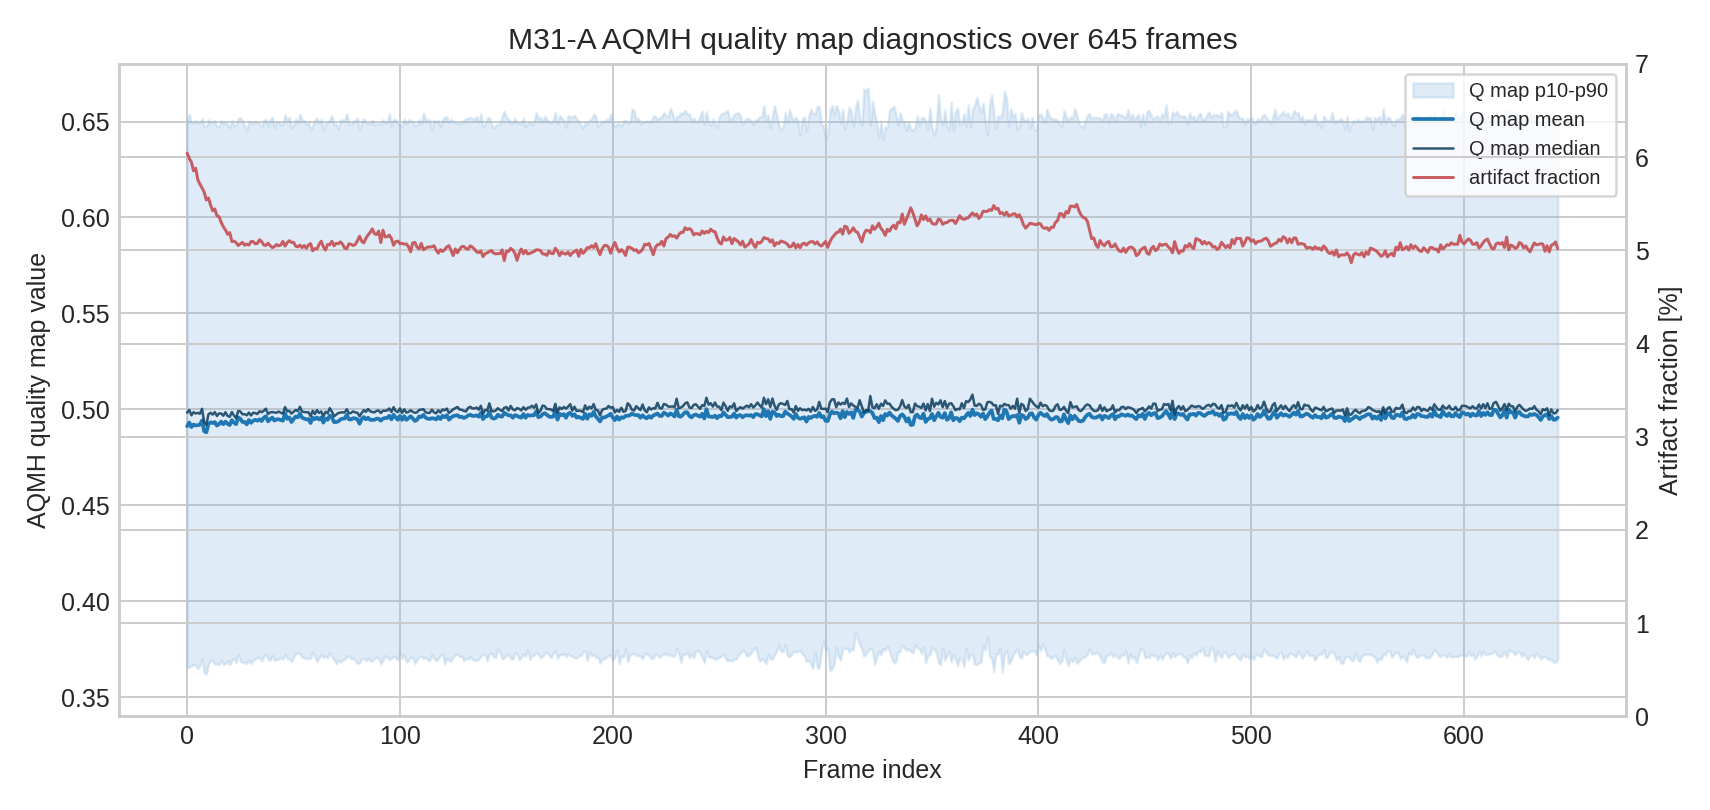
\includegraphics[width=\textwidth]{m31_aqmh_quality_timeseries.png}
\caption{Per-frame AQMH quality-map diagnostics. The shaded band shows the p10-p90 interval of
the map values; mean and median remain stable across the 645-frame sequence. The artifact
fraction stays near five percent, with a higher early-frame tail.}
\label{fig:timeseries}
\end{figure*}

\begin{figure*}[t]
\centering
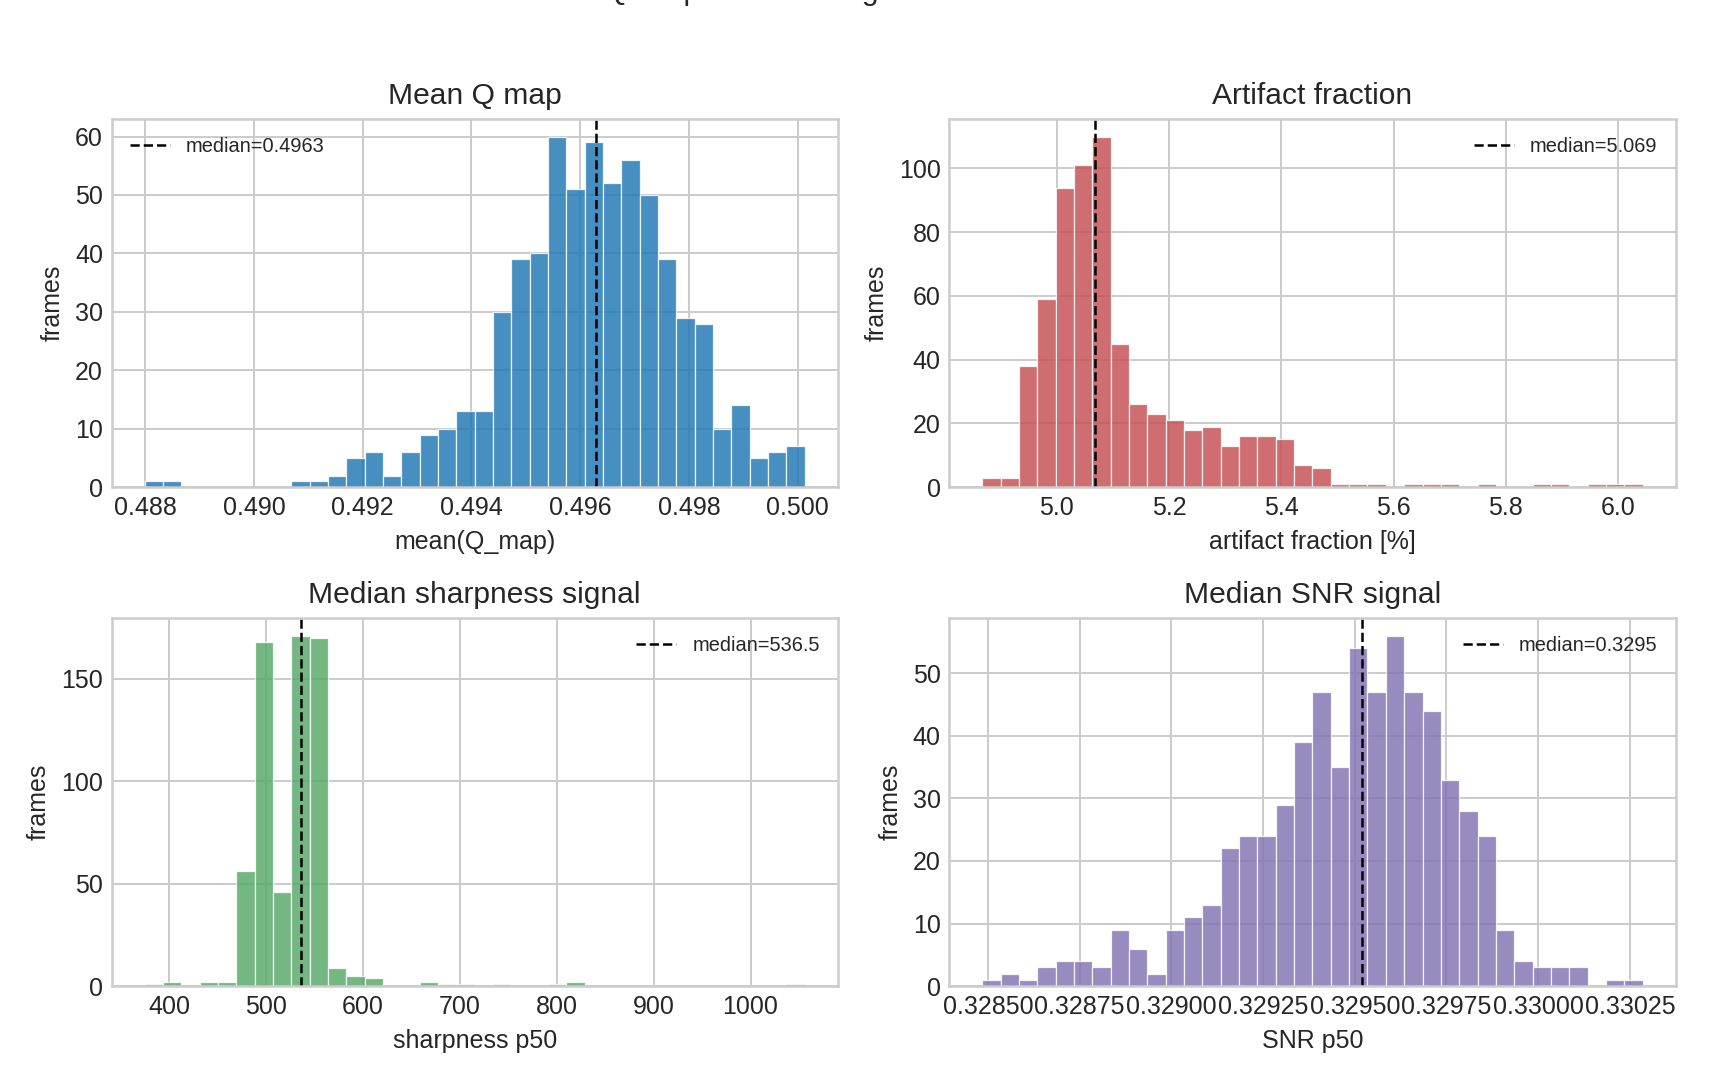
\includegraphics[width=\textwidth]{m31_aqmh_diagnostic_distributions.png}
\caption{Distributions of AQMH per-frame diagnostic quantities. The narrow quality-map mean
distribution reflects the within-frame relative normalization of the sigmoid factor; the
artifact gate remains an absolute veto term.}
\label{fig:distributions}
\end{figure*}

\subsection{Validation metrics}

The validation artifact reports an AQMH method run with both FWHM and background checks passing.
The median input seeing estimate was \num{12.351} px, while the median output FWHM was
\num{5.271} px. This corresponds to a \num{57.327}\% improvement. Background RMS changed from
\num{4.185} to \num{0.714}, reported as \num{-82.932}\%.

\begin{center}
\centering
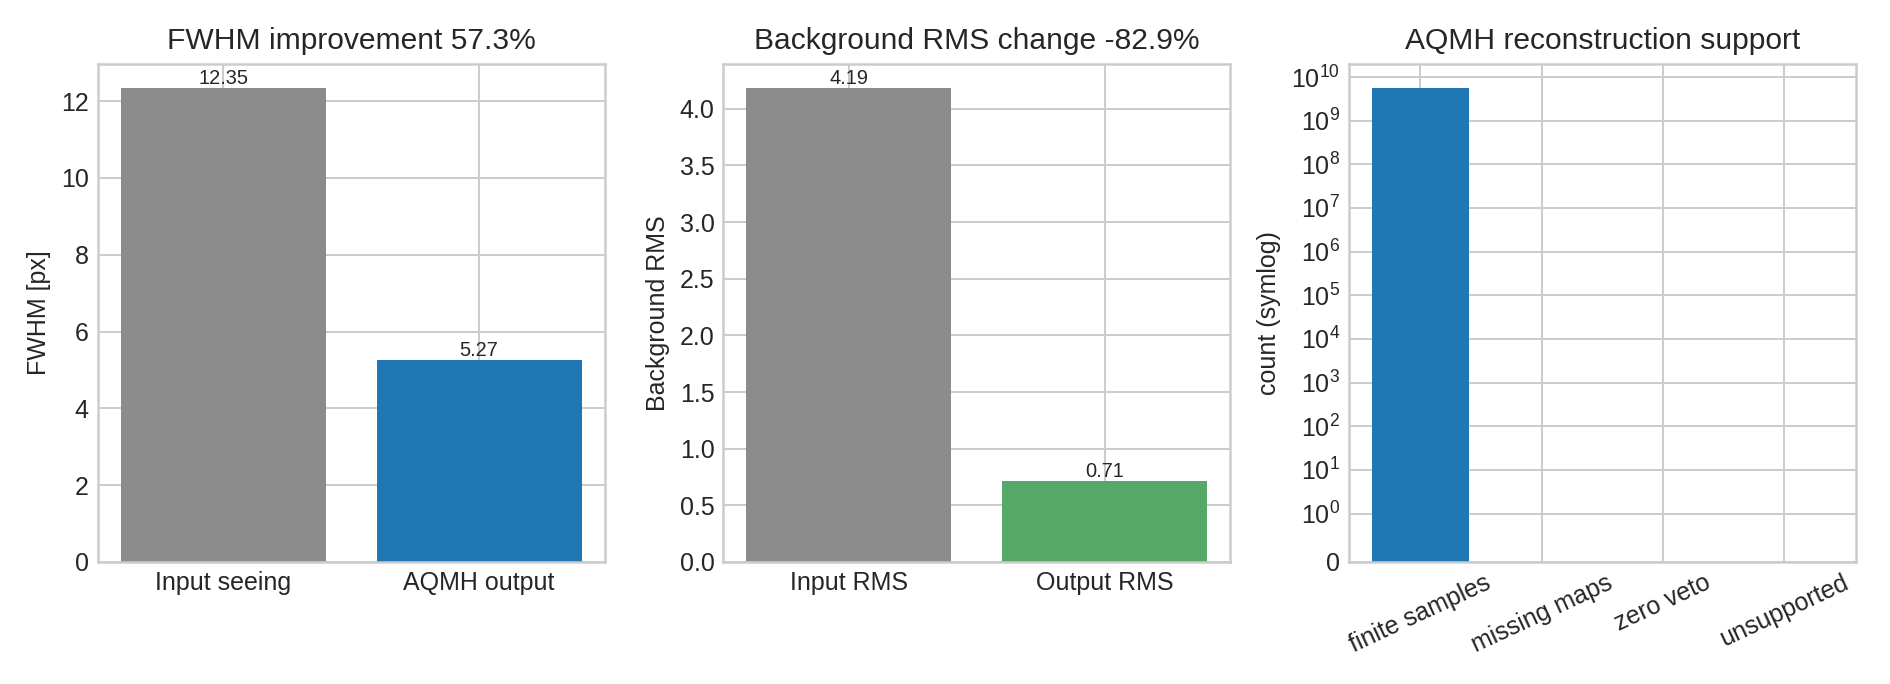
\includegraphics[width=\columnwidth]{m31_aqmh_validation_summary.png}
\captionof{figure}{Validation summary for the M31-A AQMH run. FWHM and background RMS both improve, while
the reconstruction support counters show no missing maps, unsupported pixels, or zero-veto
pixels.}
\label{fig:validation}
\end{center}

\begin{center}
\centering
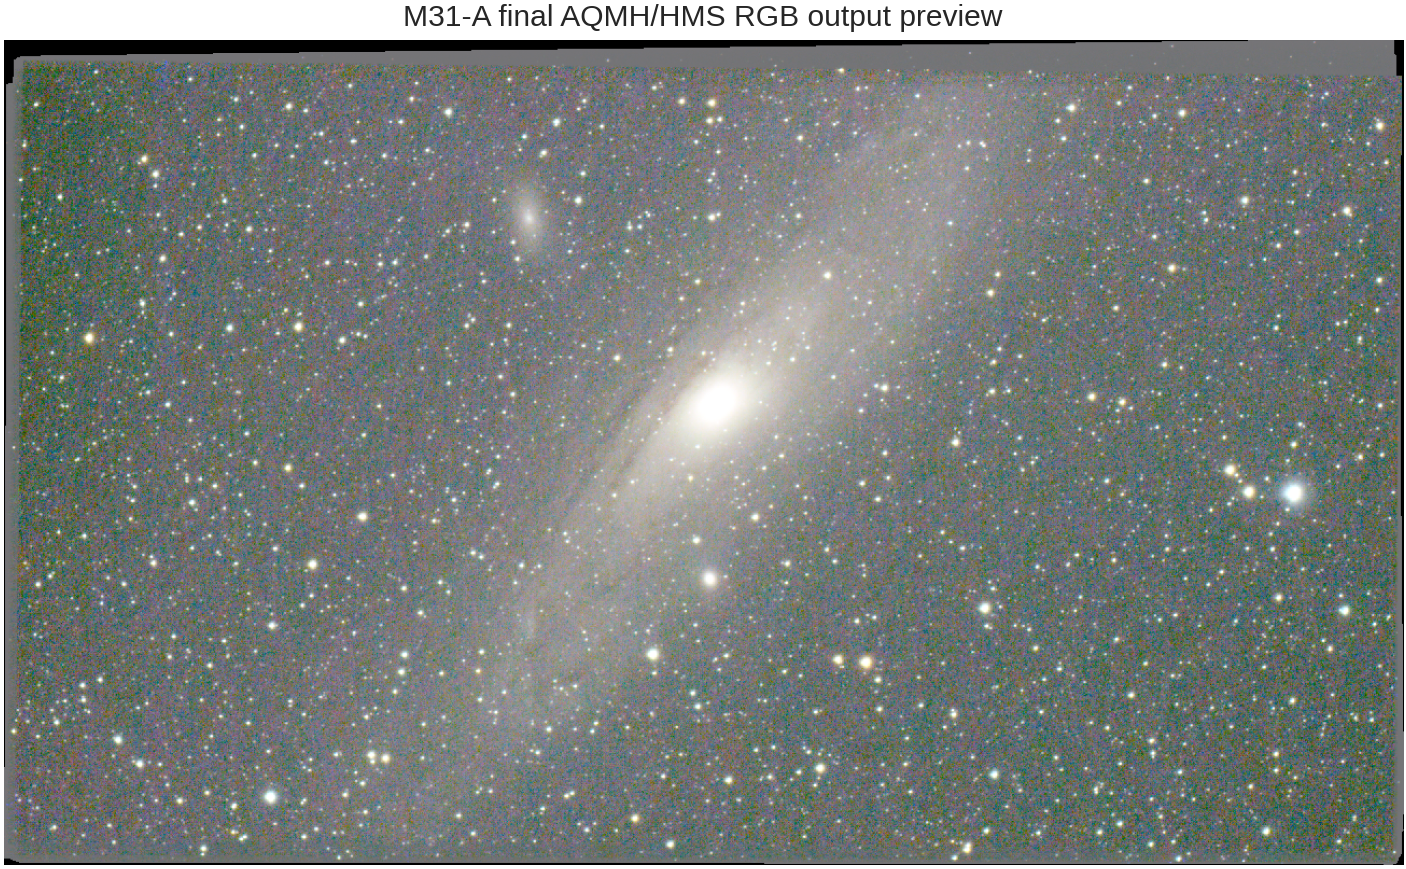
\includegraphics[width=\columnwidth]{m31_aqmh_hms_preview.png}
\captionof{figure}{Final RGB preview after AQMH reconstruction, PCC, and HMS. The preview is a visual run
product derived from the FITS output, not a quantitative measurement.}
\label{fig:preview}
\end{center}

\section{Discussion}

\subsection{What the run demonstrates}

The M31-A run demonstrates the intended AQMH execution path:
\begin{itemize}
  \item every usable frame produced a quality map;
  \item reconstruction consumed AQMH maps without classic tile-weight fallback;
  \item no quality map samples were missing during reconstruction;
  \item the output had full valid support under the run's reconstruction mask;
  \item the measured FWHM and background RMS validation metrics improved.
\end{itemize}
This is important because AQMH is not a cosmetic replacement for the classic tile phases. It is a
separate reconstruction core. The classic shared tile grid remains useful as an artifact and
geometry diagnostic, but it is not the AQMH weighting model.

\subsection{Interpretation of stable map means}

The frame-to-frame mean of $Q^{map}$ is deliberately stable. The sharpness and SNR terms are
z-normalized inside each frame, so their sigmoid contribution is mostly a within-frame relative
field. Cross-frame quality discrimination comes from the global frame weight $G_{f,c}$ and from
absolute veto terms such as the artifact gate. Therefore, a narrow distribution of map means is
not a defect; it is a consequence of separating within-frame spatial quality from between-frame
global quality.

\subsection{Limitations}

This paper reports one successful M31-A run and should not be read as a full statistical
validation across object classes, sensors, and seeing regimes. The diagnostic flag
\texttt{scene\_dependent\_snr=true} appears for all frames and deserves further evaluation: the
fallback is deterministic, but future work should quantify when background-centered local SNR
support is sufficient without the degraded-path flag. The final preview is also not a scientific
photometry product; it includes downstream PCC and HMS processing.

\section{Conclusion}

AQMH provides a deterministic pixel-wise quality-weighted alternative to coarse local tile
weighting for short-exposure deep-sky reconstruction. The M31-A run confirms that the implementation can
execute the complete AQMH path on a 645-frame dataset, write all dense quality maps, reconstruct
without classic fallback, and produce improved validation metrics. The observed FWHM improvement
of \num{57.327}\%, the absence of missing map samples, and the stable quality-map diagnostics
support the practical viability of AQMH as an independent reconstruction method in tile\_compile.

\section*{Code and Data Availability}

\textbf{Reference method.}
Classic Tile Compile is described by
\href{https://doi.org/10.5281/zenodo.19437794}{\emph{Tile-Based Quality Reconstruction for DSO},
Version 3.3.9}. The corresponding repository source is the
\href{https://github.com/jeamy/tile_compile/blob/master/docs/v3/zenodo-3.3.9/paper-tile_based_quality_reconstruction_methodology_v_3.3.9_en.tex}{v3.3.9
paper source}.

\textbf{Code.}
The public project repository is
\href{https://github.com/jeamy/tile_compile}{github.com/jeamy/tile\_compile}. AQMH method details
are documented in the
\href{https://github.com/jeamy/tile_compile/blob/master/docs/AQMH/aqmh_methodik_en.md}{AQMH
method document}.

\textbf{This paper.}
The AQMH v0.1.0 paper bundle is archived in
\href{https://github.com/jeamy/tile_compile/tree/master/docs/AQMH/zenodo-0.1.0}{docs/AQMH/zenodo-0.1.0}.
The compact values used for the tables and plots are stored in
\href{https://github.com/jeamy/tile_compile/blob/master/docs/AQMH/zenodo-0.1.0/m31_aqmh_run_summary.json}{m31\_aqmh\_run\_summary.json}.

\textbf{Run data.}
The full source measurement artifacts are local outputs from the M31-A analysis run and are not
part of the public repository bundle.

\end{document}
